\documentclass[adobefonts]{ctexart}
%\documentclass[winfonts]{ctexart}

\CTEXoptions[captiondelimiter={\quad}]


\usepackage{amsmath}            % AMS的数学宏包
\usepackage{amssymb}            % AMS的数学符号宏包
\usepackage{graphicx}           % 插入图片需要的宏包
\usepackage{float}              % 强大的浮动环境控制宏包
\usepackage{framed}             % `shaded'环境需要用到
\usepackage{enumitem}           % 增强列表功能
\usepackage{alltt}              % 在`alltt'环境中为等宽字体, 但可以使用LaTeX命令

% \usepackage{shortvrb}           % 简化\verb的写法
% \MakeShortVerb{\|}

\usepackage{listings}
\lstset{language=bash}
\lstset{extendedchars=false}
\lstset{breaklines}
\lstset{stepnumber=2}
\lstset{backgroundcolor=\color{lightgray}}


\usepackage{color}              % 可以定义各种颜色
\usepackage[x11names]{xcolor}   % 下面的RoyalBlue3颜色需要用到的宏包
% 自定义的几种颜色
\definecolor{shadecolor}{gray}{0.85}

% \definecolor{darkblue}{rgb}{52,101,164}
% \definecolor{darkgreen}{rgb}{78,154,6}

% % 设置背景颜色
% \definecolor{bisque}{rgb}{.996,.891,.755}
% \pagecolor{bisque}

\usepackage[pdfauthor={Dreamseeker},
  pdftitle={opensuse搭建ftp服务器},
  colorlinks=true,
  urlcolor=blue,
  linkcolor=RoyalBlue3]{hyperref} % 为超链接设置颜色, 修改PDF文件信息

%\CTEXsetup[name={实验,},number={\chinese{section}}]{section}


\title{\textbf{opensuse搭建ftp服务器}}
\author{deanraccoon@gmail.com}
% \date{}

\usepackage[pagestyles]{titlesec} % 定制页眉页脚
% % 设置页眉页脚
% \newpagestyle{main}{%
%   \sethead[$\cdot$~\thepage~$\cdot$][][\thesection\quad%
%   \sectiontitle]{\thesection\quad\sectiontitle}{}{%
%   $\cdot$~\thepage~$\cdot$}
%   \setfoot{}{}{}\headrule}
% \pagestyle{main}
% \renewpagestyle{plain}{\sethead{}{}{}\setfoot{}{}{}}
\pagestyle{plain}

\usepackage[top=0.75in,bottom=0.5in,left=1in,right=1in]{geometry} % 设置页边距

\setlength{\belowcaptionskip}{1em} % 设置caption之后的距离

% For LaN
\newcommand{\LaN}{L{\scriptsize\hspace{-0.47em}\raisebox{0.23em}{A}}\hspace{-0.1em}N}

\begin{document}

\maketitle
\tableofcontents

\newpage

\section{需求描述和安装vsftpd}
\subsection{需求描述}

首先假设我们有如下的需求,这个需求基本上可以覆盖一些基本需要
\begin{enumerate}
\item 有2个文件夹,一个文件夹可以匿名上传文件,叫做incoming,
  另一个叫作pub,是只读文件夹.此外,要求所有的本地用户都可以访问自己的家目录,
  并且只限制仅可以访问自己的家目录,可以读写
\item
  incoming下有一层分类目录,分别是a,b,c,配置ftp服务器,匿名用户可以在incoming/a,
  incoming/b,incoming/c这个三个文件夹中上传文件(可以带目录),但是只可以上传,不可以删除
  或者重命名已经存在的文件,保证不会来个破坏者把你的incomming文件夹弄的乱七八糟
\item
  pub文件夹下也有三个分类目录,分别是a,b,c
\end{enumerate}
这样我们的文件结构就是
\begin{figure}[htbp]
  
\includegraphics[width=6cm]{structure.eps}
\end{figure}
\subsection{安装vsftpd}
vsftpd是类unix操作系统上的ftp服务器软件,还有其他的ftp服务器软件
比如proftpd,filezilla的sever部分. proftpd与vsftpd类似,只能通过
配置文件修改配置

在opensuse上安装vsftpd非常简单
只需要一个命令
\begin{verbatim}
  sudo zypper in vsftpd
\end{verbatim}
就可以完成安装,其中sudo命令的意思是如果你的当前用户是非root用户
需要在执行这个命令的时候,提升自己的权限到root.//
如果你是在用root用户,那么就不需要敲sudo了
安装完成后用命令
\begin{verbatim}
  sudo rpm -ql vsftpd
\end{verbatim}
检查安装了哪些文件,其中/usr/sbin/vsftpd是vsftpd的二进制程序,其他/etc下的
是vsftpd的配置文件,/usr/share/下的是一些帮助文件
\subsection{第一次启动vsftpd}
启动vsftpd,检查一下安装是否正确
\begin{verbatim}
  sudo /sbin/service vsftpd start
\end{verbatim}
在默认情况下,vsftpd允许普通用户登录,比如我现在
有一个用户是opensuse,密码也是opensuse,用ftp工具
登录本机
\begin{verbatim}
  $ftp localhost
  Trying 127.0.0.1...
  Connected to localhost.
  220 (vsFTPd 2.3.2)
  Name (localhost:): opensuse
  331 Please specify the password.
  Password:
  230 Login successful.
  Remote system type is UNIX.
  Using binary mode to transfer files.
  ftp> 
\end{verbatim}
这表示已经成功地用opensuse帐户登录到本机的ftp上
默认的登录目录是opensuse的家目录.在vsftpd的默认配置下,通过ftp登录服务器的opensuse
,也可以cd到/分区,在默认情况下用户opensuse也是只读的

在linux下的ftp客户端有很多,命令行的有ftp(windows也有相同的命令),lftp(这是我个人最喜欢的ftp客户端,非常强大!),
图形界面的有gftp,filezilla.因为绝大多数linux系统无论桌面的还是服务器版的,都会装有ftp这个命令行的工具,所以
都用ftp这个工具说明.

在默认情况下,vsftpd也允许匿名用户登录
直接在命令行输入
\begin{verbatim}
  $ftp localhost
  Trying 127.0.0.1...
  Connected to localhost.
  220 (vsFTPd 2.3.2)
  Name (localhost:): anonymous
  331 Please specify the password.
  Password:
  230 Login successful.
  Remote system type is UNIX.
  Using binary mode to transfer files.
  ftp> 
\end{verbatim}
在询问用户名和密码的时候,直接输入anonymous,密码为空,直接回车
就可以登录了.也可以用户名ftp,密码ftp登录,也表示自己是匿名用户
匿名用户默认的登录地址也是在ftp的家目录中,查看/etc/passwd文件
可以看到ftp的家目录在/srv/ftp下,那么匿名用户登录的初始位置就在
/srv/ftp中

下面就看看如何配置vsftpd达到需求的效果


\section{配置vsftpd}
\subsection{pub文件夹配置}
在pub文件夹下建立三个子文件夹,a,b,c
把需要的文件直接用拷贝到各个需要的文件夹就OK了
就这么简单!

这是因为root的umask是022,
\begin{verbatim}
  linux-lp6d:~ # umask 
  0022
\end{verbatim}
也就是说root建立的文件夹,默认
权限是755(其他用户可读,可搜索,不可写),建立的文件权限是
644(其他用户只读),这样既保证了ftp用户可以下载,浏览这些文件,又
不能修改这些文件

还有一种常见的情况.就是ftp里的文件就在服务器的其他地方或者在网络的其他地方,
如果再拷贝一次实在是太浪费硬盘了,出现这种情况,只需要把文件系统或者远程的网络
挂载(mount)到,a,b,c其中一个文件夹下就可以了,只要保证文件权限是只读就可以了,
就是一般的755的文件权限
比如我们有很多数据在/home/data下,/home/data的属主是root.
用mount命令把/home/data挂载到/srv/ftp/a上就大功告成
\begin{verbatim}
  $sudo mount --bind /home/data/ /srv/ftp/pub/a/
\end{verbatim}
这样访问a文件夹的时候就可以看到/home/data下面的内容了,--bind是说明把已经mount在文件系统
中的一部分文件夹再重新mount到另一块文件系统中,让它可以访问。有点儿类似于ln。这个需求也可以用ln
实现

NFS方式也类似,NFS可以把网络上开启NFS服务的计算机硬盘挂在到本地,如同本地文件一样
操作,比如把远程192.168.1.1的/home/data文件夹挂载到本地/srv/ftp/pub/b上,假设192.168.1.1
上的NFS服务器已经开启
\begin{verbatim}
  $sudo mount -t nfs 192.168.1.1:/home/data/ /srv/ftp/pub/b
\end{verbatim}

总的来说,配置匿名ftp只读就很容易,连vsftpd的配置文件都不用修改!
只要管好这些文件的权限就可以了,vsftpd就可以提供了高效安全的服务
\subsection{incomming文件夹配置}
incomming文件夹要配置ftp帐户可写,就需要改一改vsftpd的配置文件了,通常是/etc/vsftpd.conf,其实这也非常
简单,因为vsftpd的配置文件有非常多的注释,看注释就可以看懂
首先要确保打开匿名ftp的下面几个选项
\begin{enumerate}
\item write\_enable=YES     \#运行FTP用户(包括匿名用户和可登录用户)的写操作
\item anonymous\_enable=YES \#允许匿名FTP,默认YES
\item anon\_world\_readable\_only=YES \#允许匿名用户下载全局可读的文件,默认YES
\item anon\_upload\_enable=YES \#允许匿名用户上传文件,默认NO
\end{enumerate}
确保这四个选项打开,并重启vsftpd
再加上之后一个重要的操作,就可以实现匿名用户上传文件了

这个重要的操作就是:用chmod修改incomming下a,b,c三个文件夹的其他用户可写权限,在Linux
中文件夹的可写权限表示可在这个文件夹下新增,修改文件
文件夹现在的权限是
\begin{figure}[htbp]
  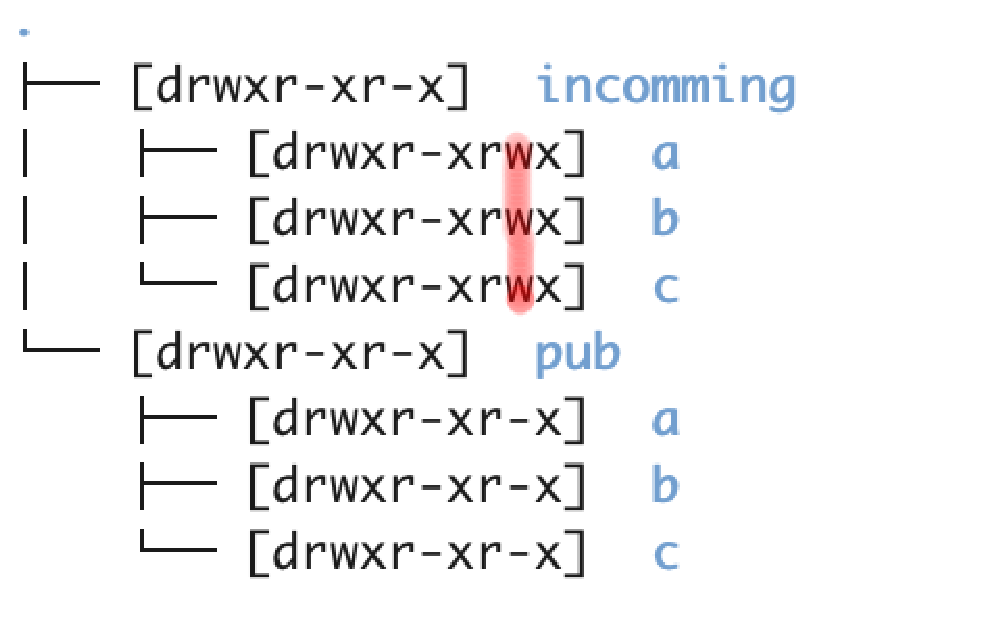
\includegraphics[width=6cm]{perm.eps}
\end{figure}
所有文件夹的owner是root,只修改了红色的部分--其他用户可写,让incomming下的a,b,c三个文件夹可以
上传文件,是不是很简单?

总结一下,vsftp配置匿名用户上传,只需要打开配置文件里的4个选项,并且修改文件夹的权限,就可以实现匿名上传了。
而匿名下载就更简单了,通过查看/etc/passwd(因为不同linux发行版,ftp用户的家目录不一定相同)找到匿名用户的家目录,
确保权限正确--ftp用户有可读权限,无可写权限就可以了,就想pub文件夹的权限一样就可以了
\subsection{匿名用户其他配置说明}

\begin{itemize}
    \item anon\_umask=022                \#匿名用户上传后的文件权限,默认是700,除了ftp用户以外,别人不能访问,最好是改成755,强烈推荐打开
    \item anon\_mkdir\_write\_enable=YES \#运行匿名用户在可写权限的文件夹里建立文件,这样就允许匿名用户上传文件夹了,推荐打开
	\item anon\_other\_write\_enable=YES \#匿名用户在可写的文件夹里面,不仅可以上传还可以删除,修改文件,建议不要打开,防止有人乱删东西
    \item chown\_uploads=YES              \#匿名用户上传文件后,文件的owner还是ftp这个用户,可以修改成其他用户为属主,这个选项和下面的一个选项共同作用,修改ftp用户上传的文件的属主        
	\item chown\_username=whatever        \#官方推荐修改owner可以,但是不要把文件owner设为root
\end{itemize}

\subsection{本地用户登录}
在前面说过,默认情况下vsftpd允许系统用户登录服务器, 比如opensuse用户
可以通过ftp访问服务器,并且不受家目录的限制,可以访问根分区等等。
下面就介绍一些vsftpd的配置文件,修改这些行为
\begin{itemize}
    \item local\_enable=YES     \#允许本地用户登录,系统默认是YES,如果改成NO的话,像opensuse用户就没有办法登录了
    \item chroot\_local\_user=YES  \#限制本地用户只能在自己的家目录,这个配置成YES的话,用户就不能到处跑了,很多虚拟主机都是这么做的
\end{itemize}

\section{其他}
vsftpd默认是不打开日志的,如果空间允许,还是建议打开log功能
其他选项比如idle时间,都可以按照自己的需要配置

总的来说,vsftpd的配置还是比较简单的,还有vsftpd配合mysql实现虚拟用户可以参考其他文档:)
,如果自己建立的ftp不能登录,可以这样逐步排查
\begin{enumerate}
\item 检查vsftpd是否启动,坚持21端口是否打开
\item 检查防火墙是不是封了ftp端口,用iptables命令
\item ftp localhost自己登录自己的ftp
\item 如果本机可以登录,说明就是网络或者防火墙的问题了
\end{enumerate}
\input{../readme}
\end{document}
